% write your paper in here

\chapter{Scaffolding assemblies with Hi-C}

Recent genome assembly projects generally aim to achieve chromosome-level scaffolds, and Hi-C scaffolding is a major step to reach this goal. This method has been included successfully in many studies for bacteria, yeasts, plants, animals, and is part of assembly pipelines for several consortia, such as the Vertebrate Genome Project \cite{vgp} and the Darwin Tree of Life \cite{dtol}. instaGRAAL is an overhauled, improved version of GRAAL \cite{graal}, a Hi-C scaffolder inspired by Gibbs sampling, a MCMC-based approach, to iteratively test and ponder arrangements of DNA fragments until the resulting organization converges towards an assembly with a higher likelihood based on contact frequencies. Two main aspects were improved: first, instaGRAAL, through the use of sparse contact maps, is more computationally efficient, enabling it to handle larger genomes (over 1 Gb); second, it introduces a module to automatically refine the scaffolds based on the input contigs, and reduce local misassemblies. In the following paper, instaGRAAL was used to assemble the brown algae \textit{Desmarestia herbacea} and \textit{Ectocarpus} sp., and benchmarked against SALSA2 \cite{salsa2} on a human; it systematically yielded chromosome-level scaffolds. \\
I contributed to testing instaGRAAL, in particular regarding its application to the human genome. I also improved the documentation to make it more accessible for new users, and contribute since then to the maintenance of the program on the github account of Romain Koszul's lab  \href{https://github.com/koszullab/instaGRAAL}{github.com/koszullab/instaGRAAL}. \\

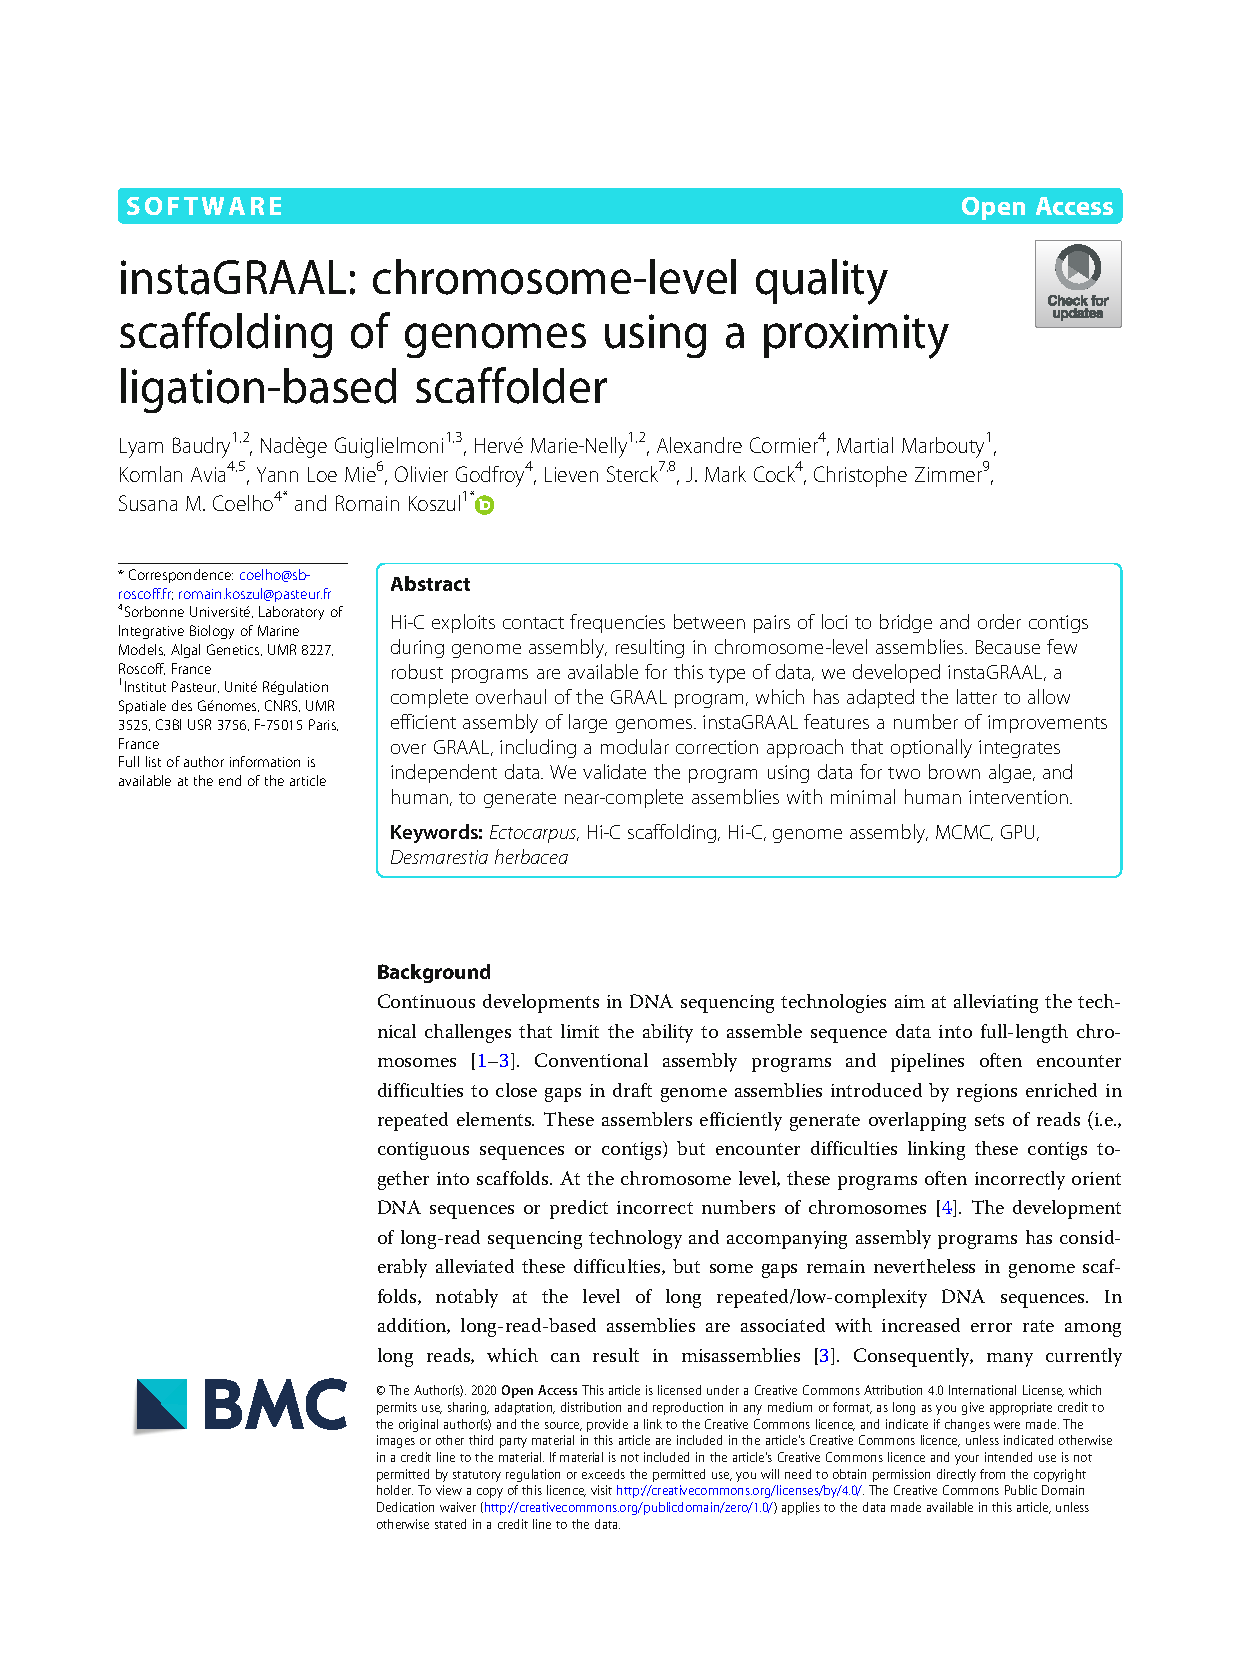
\includepdf[pages=-, pagecommand={}]{articles/instagraal.pdf}

\begin{suppsection}
\beginsupplement

\begin{table}[ht]
\centering
\caption{Example of a sparse matrix.}
\begin{tabular}{|c|c|c|}
\hline
\textbf{id\_frag\_a} & \textbf{id\_frag\_b} & \textbf{n\_contacts} \\
\hline
0 & 0 & 1368 \\
0 & 1 & 21 \\
0 & 2 & 7 \\
0 & 3 & 3 \\
0 & 4 & 5 \\
0 & 7 & 5 \\
0 & 8 & 1 \\
0 & 9 & 1 \\
0 & 12 & 2 \\
0 & 15 & 1 \\
0 & 22 & 1 \\
0 & 23 & 1 \\
0 & 26 & 1 \\
0 & 27 & 1 \\
0 & 33 & 2 \\
0 & 36 & 2 \\
0 & 37 & 1 \\
0 & 51 & 1 \\
0 & 69 & 1 \\
0 & 74 & 2 \\
0 & 76 & 1 \\
0 & 97 & 1 \\
0 & 99 & 1 \\
0 & 107 & 1 \\
\hline
\end{tabular}
\label{tab:t1}
\end{table}

\begin{table}[ht]
\centering
\caption{Comparison of the integrated sequences between the different assemblies and the v1 assembly for \textit{Ectocarpus} sp.}
\begin{tabular}{|l|c|c|c|}
\hline
    & \textbf{v1 assembly} & \textbf{linkage group} & \textbf{corrected instaGRAAL} \\
    &  & \textbf{v2 assembly} & \textbf{v4 assembly} \\
\hline
Scaffolds integrated into linkage & 325 & 531 & 793 \\
groups (out of 1561) &  &  &  \\
\hline
Percent sequence data integrated & 70.10\% & 90.50\% & 96.80\% \\
into linkage groups &  &  &  \\
\hline
Integrated oriented scaffolds in & 12\% & 49\% & 100\% \\
the linkage groups &  &  &  \\
\hline
Number of linkage groups & 34 & 28 & 27 \\
\hline
\end{tabular}
\label{tab:t2}
\end{table}

\begin{table}[ht]
\centering
\caption{Correspondences between instaGRAAL super scaffolds and linkage groups from the v2 assembly for the \textit{Ectocarpus} sp. genome.}
\begin{tabular}{|c|c|}
\hline
\textbf{instaGRAAL} & \textbf{Linkage group} \\
\textbf{v4 assembly} & \textbf{v2 assembly} \\
\hline
1 & 1 \\
2 & 21 \\
3 & 4 \& 28 \\
4 & 5 \\
5 & 13 \\
6 & 6 \\
7 & 12 \\
8 & 7 \\
9 & 27 \\
10 & 26 \\
11 & 3 \\
12 & 2 \\
13 & 8 \\
14 & 14 \\
15 & 10 \\
16 & 11 \\
17 & 19 \\
18 & 16 \\
19 & 9 \\
20 & 15 \\
21 & 18 \\
22 & 20 \\
23 & 24 \\
24 & 23 \\
25 & 17 \\
26 & 25 \\
27 & 22 \\
\hline
\end{tabular}
\label{tab:t3}
\end{table}

\begin{table}[ht]
\centering
\caption{Metrics of \textit{Desmarestia herbacea} assemblies using three different programs.}
\begin{tabular}{|l|c|c|c|c|}
\hline
    & \textbf{\textit{De novo} original assembly} & \textbf{3D-DNA} & \textbf{SALSA2} & \textbf{instaGRAAL} \\
\hline
N50 (bp) & 184,092 & 175,000 & 12,780,148 & 12,444,485 \\
L50 & 697 & 545 & 11 & 17 \\
Contig count & 7,743 & 5,385 & 4,827 & 4,304 \\
BUSCO \% & 72.6 & 70.7 & 73.6 & 73.0 \\
\hline
\end{tabular}
\label{tab:t4}
\end{table}

\begin{table}[ht]
\centering
\caption{Performance of GRAAL and instaGRAAL at scaffolding the \textit{Ectocarpus} sp. genome. }
\begin{tabular}{|l|c|c|}
\hline
    & \textbf{GRAAL} & \textbf{instaGRAAL} \\
\hline
Peak memory load (Gb) & 2.5 & 1.1 \\
Memory used in graphic card & 113 (Mb) & 11 \\
Per-cycle runtime (avg. over 20 min) & 13 & 4 \\
\hline
\end{tabular}
\label{tab:t5}
\end{table}

\begin{figure}[ht]
\centering
    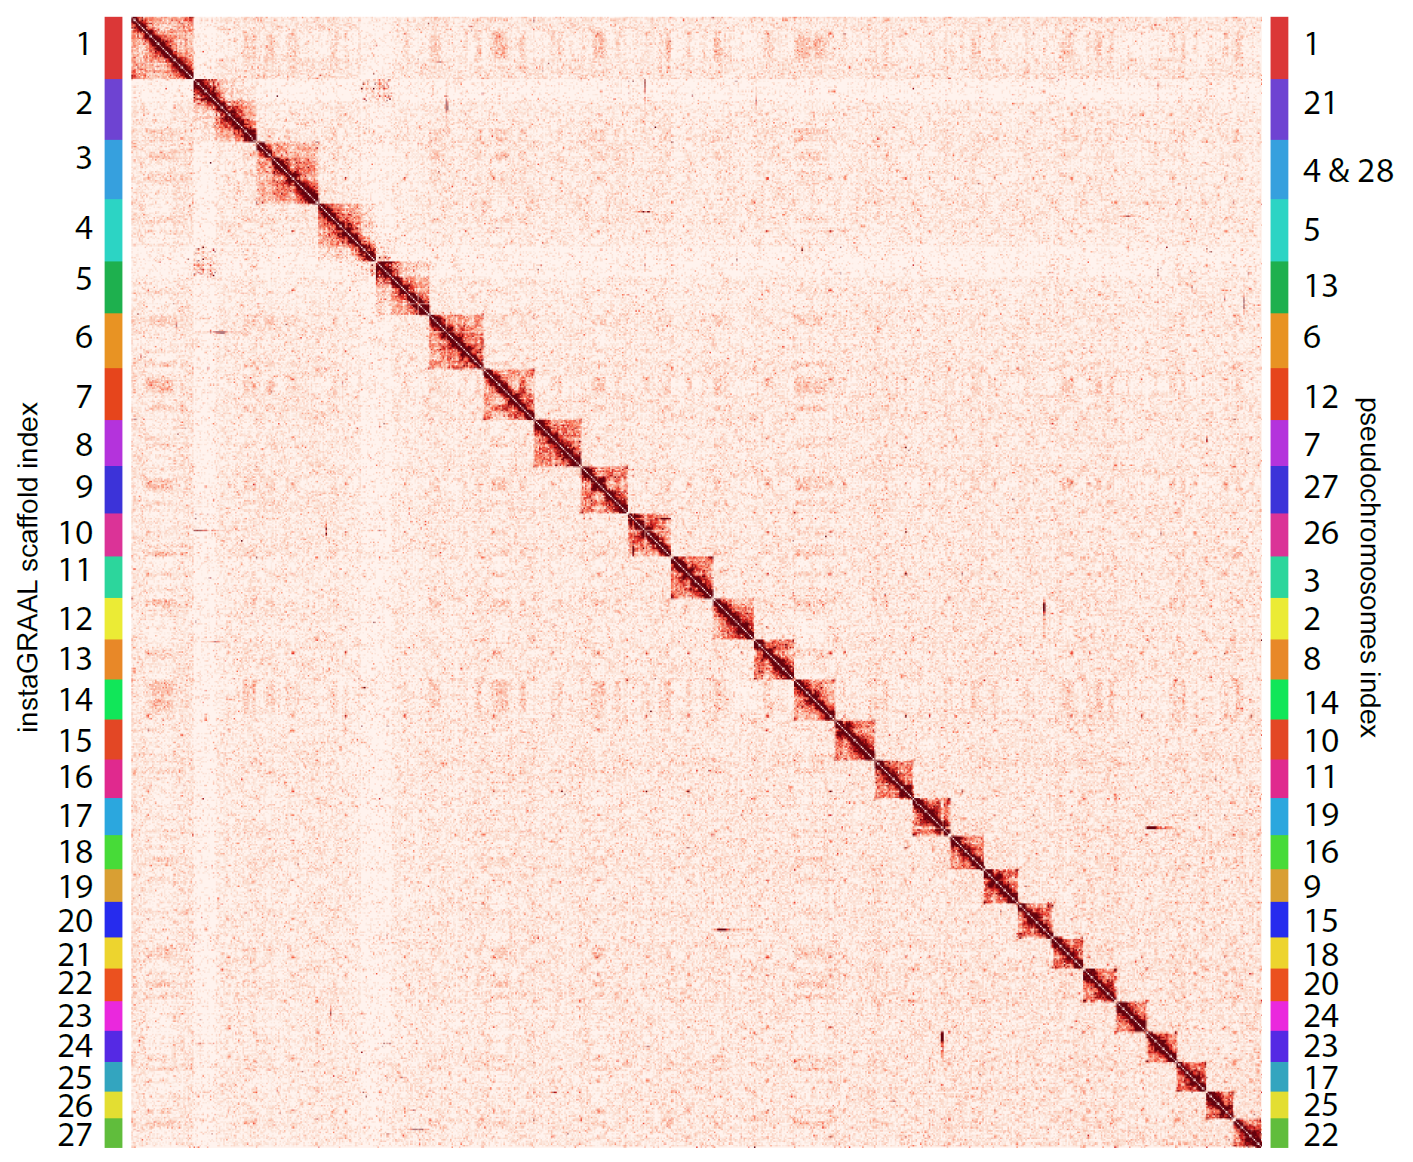
\includegraphics[width=13.5cm]{fig/instagraal/s1.png}
    \caption{Normalized contact map of the \textit{Ectocarpus} sp. genome scaffolded using instaGRAAL (bin = 200 kb). The colour scale represents the normalized interaction frequencies. No large-scale rearrangements are clearly apparent in the interchromosomal contacts. On the right the linkage groups indices from the v2 assembly are indicated.}
    \label{fig:instagraal_s1}
\end{figure}

\begin{figure}[ht]
\centering
    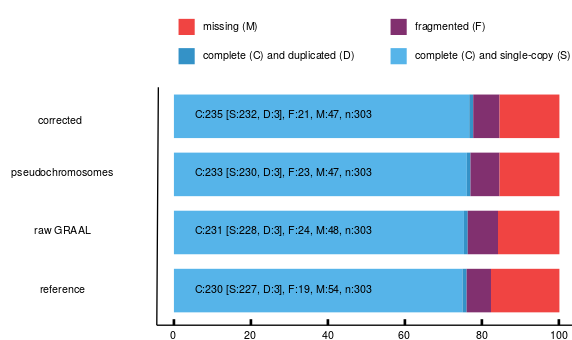
\includegraphics{fig/instagraal/s2.png}
    \caption{Estimates of BUSCO completeness for the three \textit{Ectocarpus} sp. assemblies and the reference genome v1 assembly.}
    \label{fig:instagraal_s2}
\end{figure}

\begin{figure}[ht]
\centering
    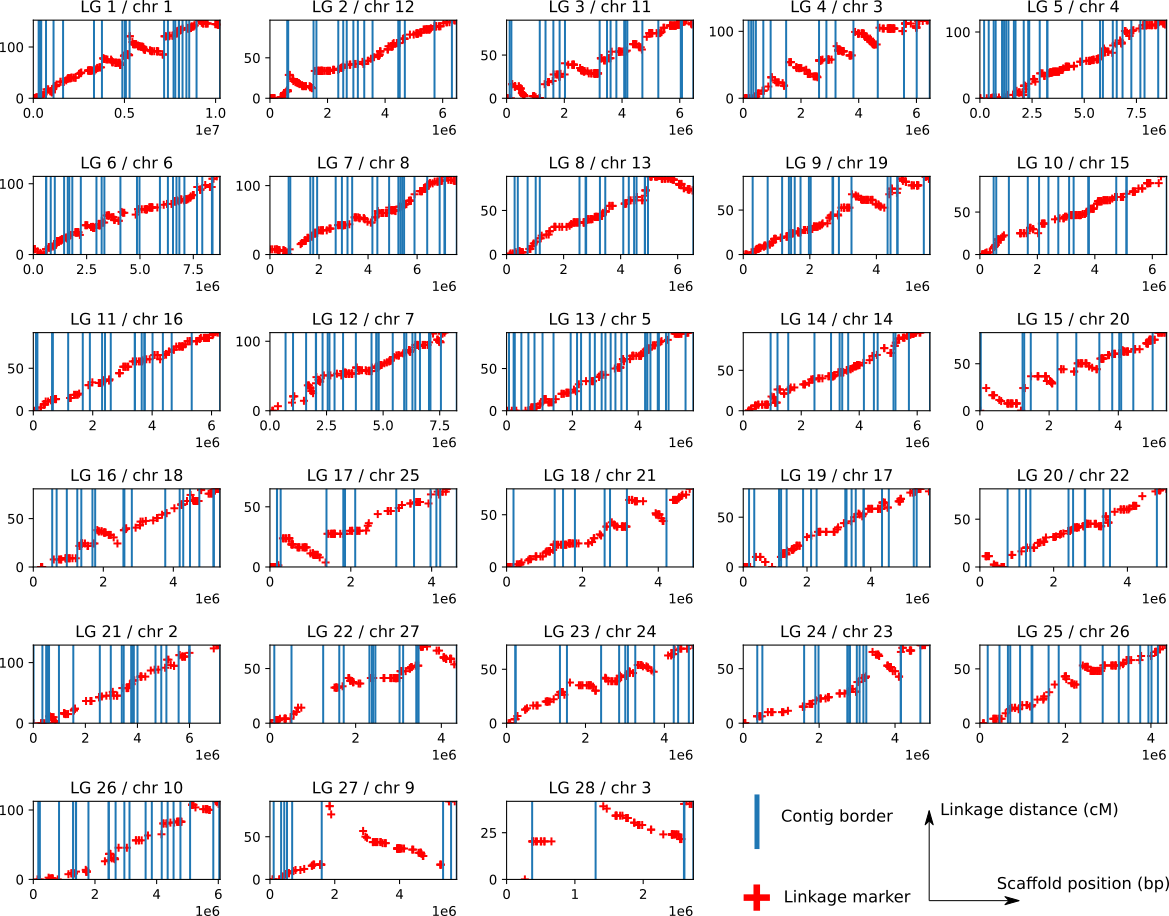
\includegraphics[width=13.5cm]{fig/instagraal/s3.png}
    \caption{Linkage markers vs. scaffold positions for all linkage groups/chromosomes (chromosome 3 is made up of linkage groups 4 and 28). The initial contig borders within each chromosome have been underlined. Linkage marker positions are always monotonous (only increasing, or only decreasing) within an initial contig.}
    \label{fig:instagraal_s3}
\end{figure}

\begin{figure}[ht]
\centering
    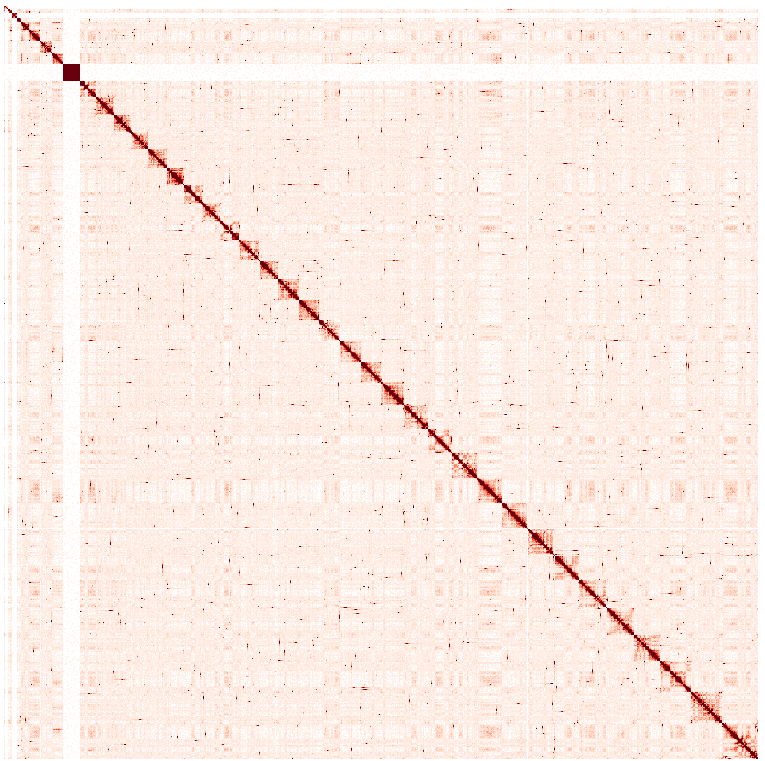
\includegraphics[width=13.5cm]{fig/instagraal/s4.png}
    \caption{The 40 main scaffolds of \textit{Desmarestia herbacea} after instaGRAAL scaffolding.}
    \label{fig:instagraal_s4}
\end{figure}

\begin{figure}[ht]
\centering
    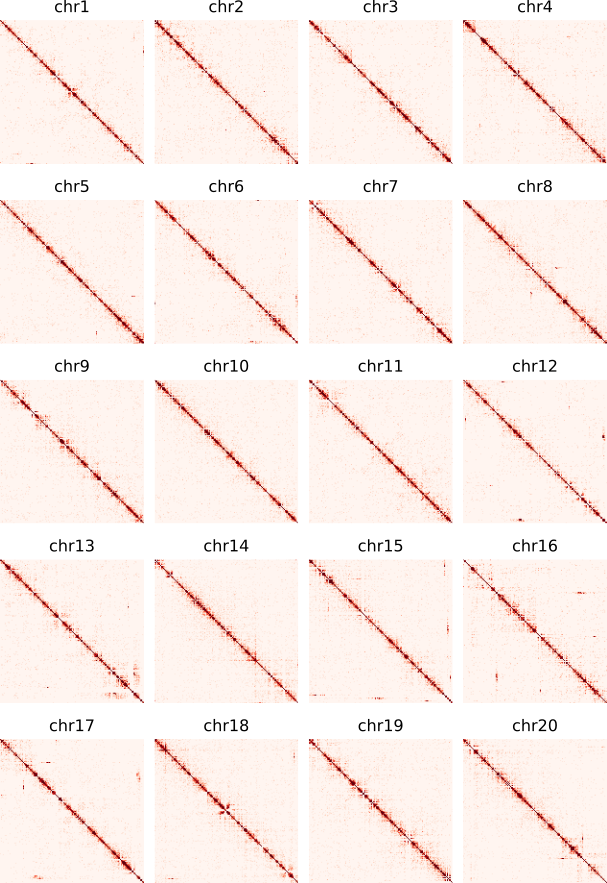
\includegraphics[width=13.5cm]{fig/instagraal/s5.png}
    \caption{Contact maps of the first twenty newly formed scaffolds/putative chromosomes of \textit{Desmarestia herbacea}, generated after scaffolding at a 20-kb resolution.}
    \label{fig:instagraal_s5}
\end{figure}

\begin{figure}[ht]
\centering
    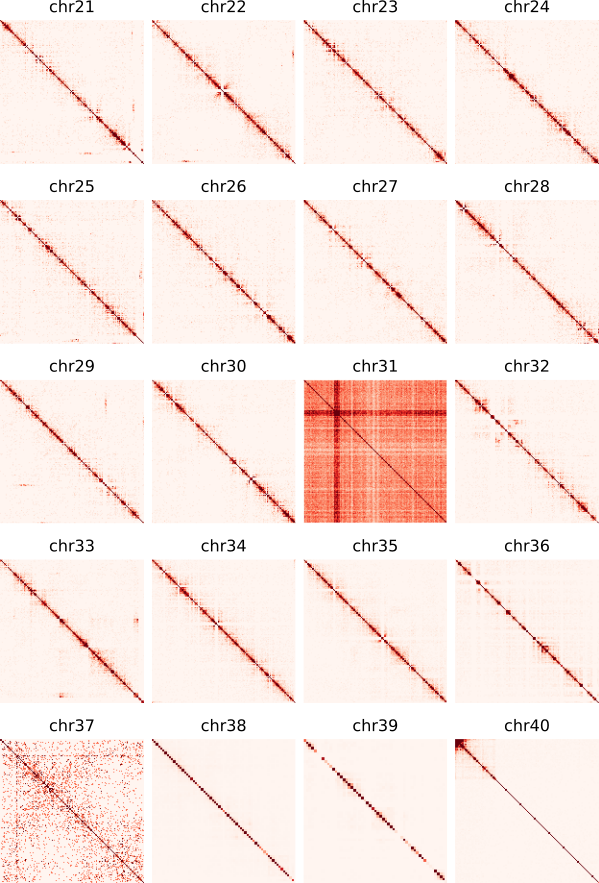
\includegraphics[width=13.5cm]{fig/instagraal/s6.png}
    \caption{The last twenty newly formed scaffolds/putative chromosomes of \textit{Desmarestia herbacea} post-scaffolding at a 20-kb resolution.}
    \label{fig:instagraal_s6}
\end{figure}

\begin{figure}[ht]
\centering
    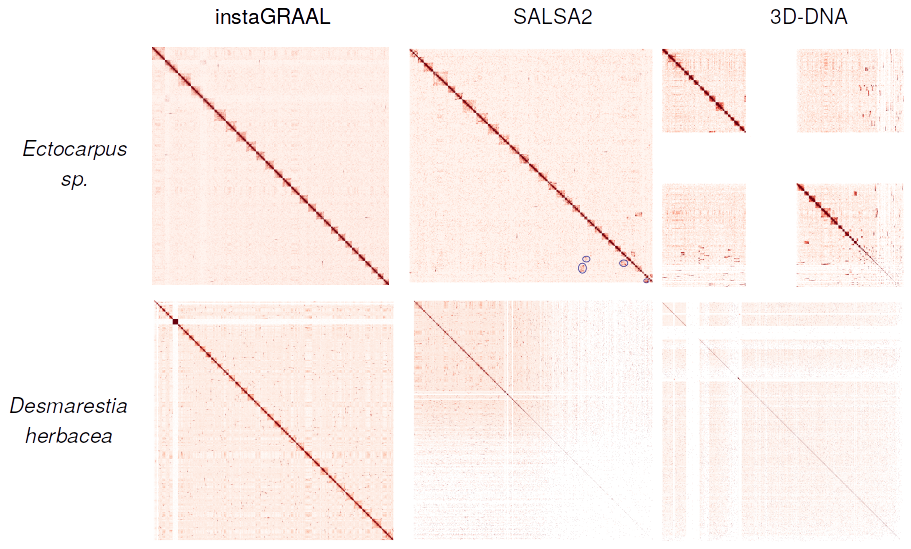
\includegraphics[width=13.5cm]{fig/instagraal/s7.png}
    \caption{Normalized contact map of the \textit{Ectocarpus} sp. genome scaffolded using instaGRAAL (bin = 200 kb). The colour scale represents the normalized interaction frequencies. No large-scale rearrangements are clearly apparent in the interchromosomal contacts. On the right the linkage groups indices from the v2 assembly are indicated.}
    \label{fig:instagraal_s7}
\end{figure}

\begin{figure}[ht]
\centering
    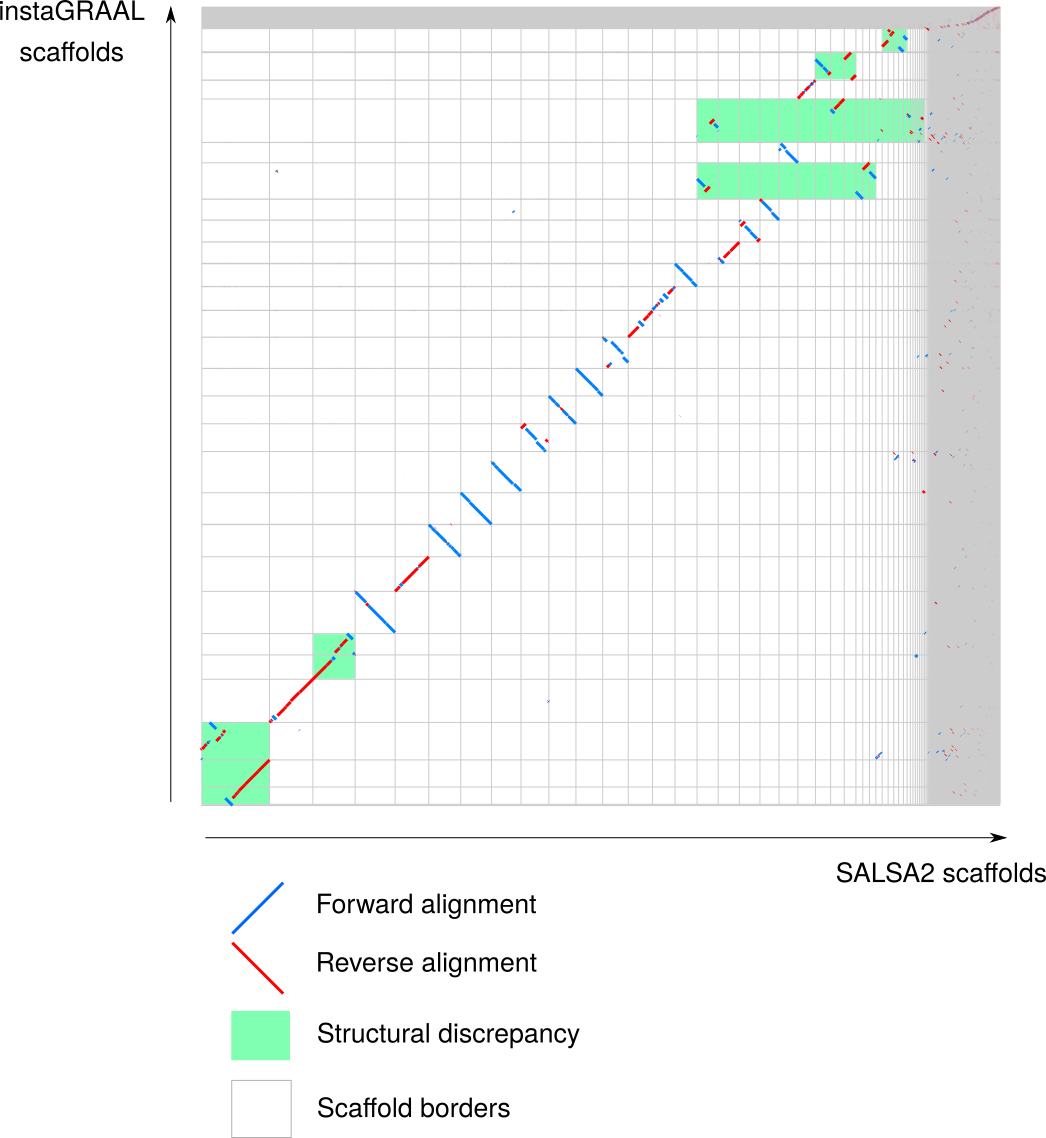
\includegraphics[width=13.5cm]{fig/instagraal/s8.png}
    \caption{Similarity dotplot of the SALSA2 vs. instaGRAAL 27 scaffolds for \textit{Ectocarpus} sp. large-scale structural discrepancies have been underlined in green. The contact maps suggest instaGRAAL solutions are more likely. }
    \label{fig:instagraal_s8}
\end{figure}

\begin{figure}[ht]
\centering
    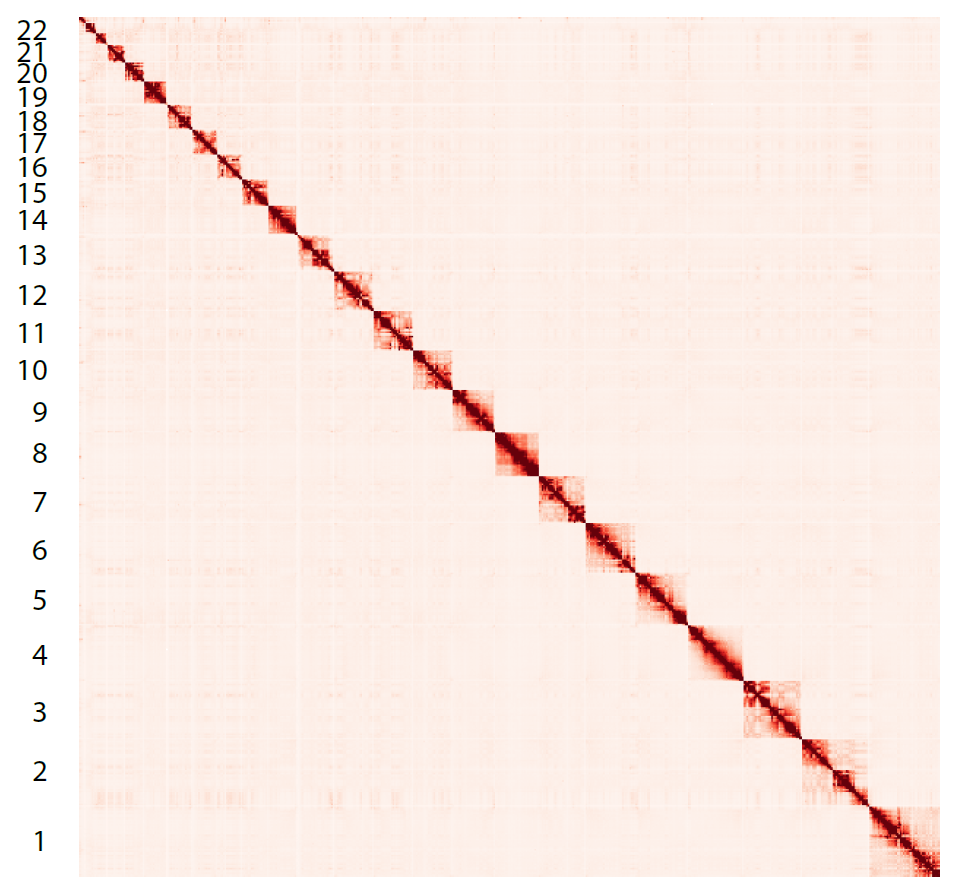
\includegraphics[width=13.5cm]{fig/instagraal/s9.png}
    \caption{Contact map of the \textit{Homo sapiens} genome, fragmented in 300 kb sequences, after scaffolding with instaGRAAL, at 5-Mb resolution.}
    \label{fig:instagraal_s9}
\end{figure}

\begin{figure}[ht]
\centering
    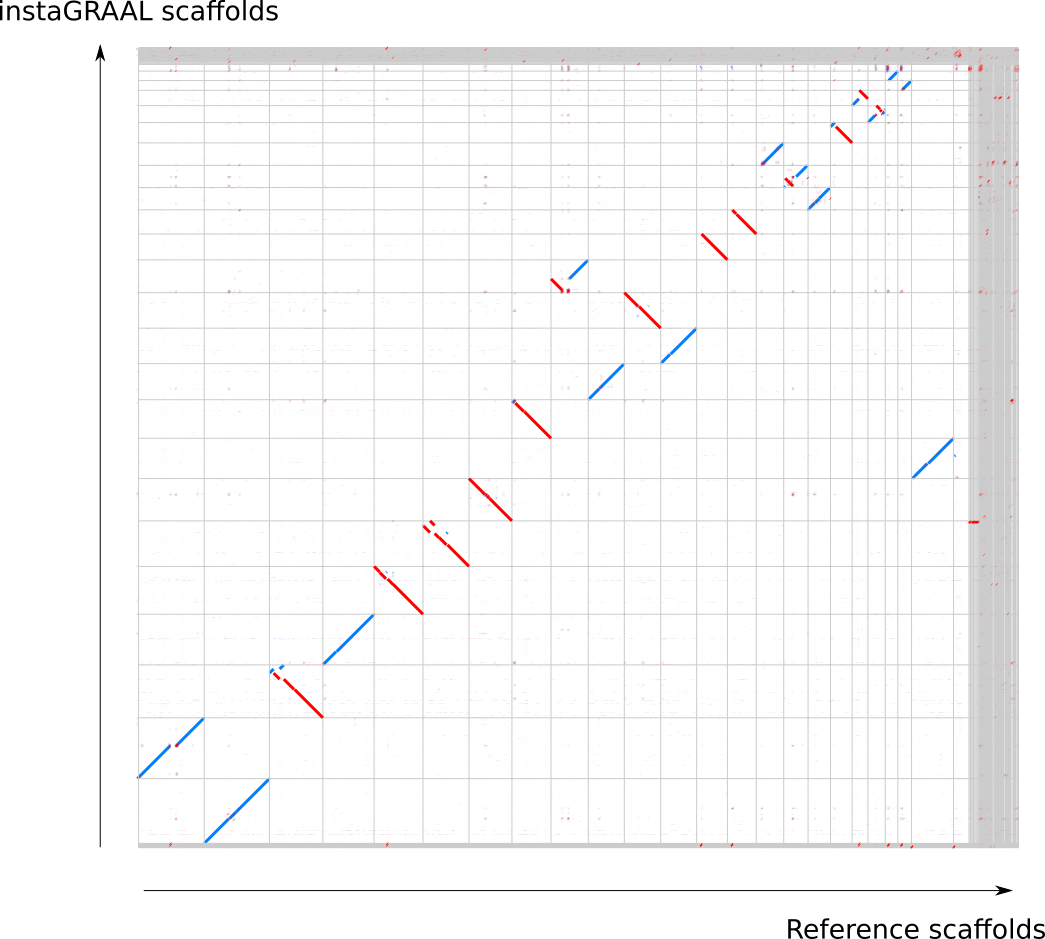
\includegraphics[width=13.5cm]{fig/instagraal/s10.png}
    \caption{Similarity dotplot of the instaGRAAL vs. reference scaffolds for the GRCh38 human genome. Relocations are visible but the one-to-one mapping between the 23 first scaffolds is preserved.}
    \label{fig:instagraal_s10}
\end{figure}

\begin{figure}[ht]
\centering
    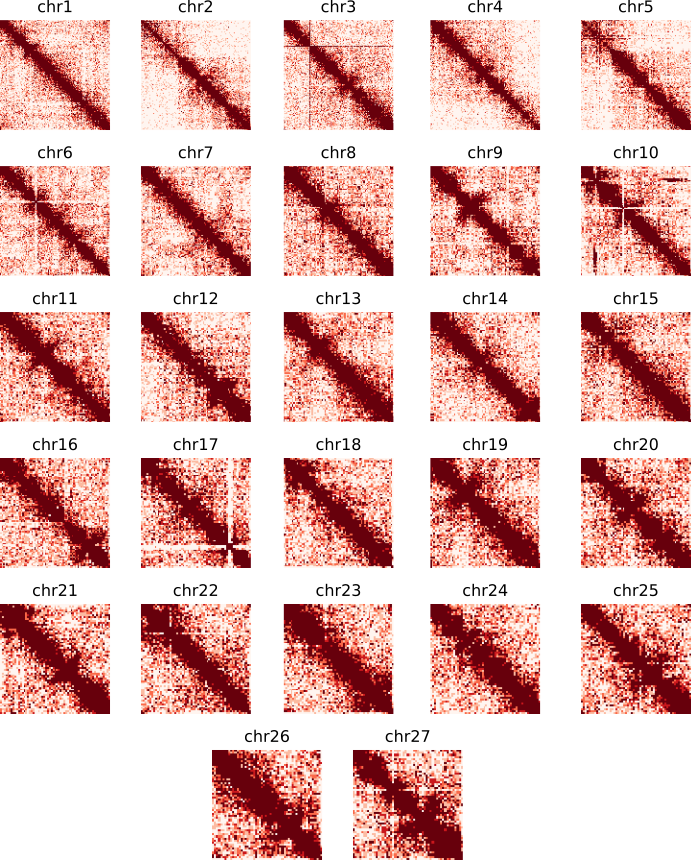
\includegraphics[width=13.5cm]{fig/instagraal/s11.png}
    \caption{All 27 newly formed scaffolds/putative chromosomes of \textit{Ectocarpus} sp. post-scaffolding at a 50-kb resolution. Centromere patterns are clearly apparent in all chromosomes, but some errors (potentially due to mapping issues) linger, such as chromosome 10 or 17.}
    \label{fig:instagraal_s11}
\end{figure}

\end{suppsection}